\documentclass[11pt]{article}

\usepackage[margin=1in]{geometry}
\usepackage{amsmath, amssymb}
\usepackage{graphicx}
\usepackage{caption}
\usepackage{subcaption}
\usepackage{enumitem}
\usepackage{hyperref}
\usepackage{fancyhdr}
\usepackage{titlesec}
\usepackage{booktabs}
\usepackage{float}
\usepackage[section]{placeins}
\pagestyle{fancy}
\fancyhf{}
\rhead{ML Project 7 Report}
\cfoot{\thepage}

\titleformat{\section}{\large\bfseries}{\thesection}{1em}{}
\titleformat{\subsection}{\normalsize\bfseries}{\thesubsection}{1em}{}
\setlength{\parskip}{3pt}
\setlength{\floatsep}{6pt}
\setlength{\textfloatsep}{6pt}
\setlength{\intextsep}{6pt}


\title{\vspace{-1.5cm}\textbf{Project 7: Forecasting Electricity Load\\
with Time-Based Fourier Features}}
\author{Maria Akhankova, Leon Lorenz \\
Applied Machine Learning in Python - LMU \\
\texttt{M.Akhankova@campus.lmu.de, Leon.Lorenz@campus.lmu.de}}
\date{\today}

\begin{document}

\maketitle
\thispagestyle{fancy}


\section{Task Overview}

Electricity consumption follows strong periodic patterns shaped by daily routines, weekly schedules, and seasonal cycles. The goal is to predict hourly electricity demand $y_t$ (in kilowatts) using only calendar time:
\[
\hat{y}_t = f\bigl(\text{hour}(t),\ \text{dayofweek}(t),\ 
\text{dayofyear}(t)\bigr)
\]

\textbf{Dataset.} We use the UCI Individual Household Electric Power Consumption dataset, containing minute-level readings from a single household in France (December 2006 - November 2010). We focus on \texttt{Global\_active\_power} (kW), resampled to hourly resolution, yielding 34{,}168 observations after removing missing values.

\textbf{Challenges.} Time is a circular variable (hour 23 and hour 0 are adjacent but numerically far apart) requiring special encoding. The dataset also contains unpredictable spikes from individual appliance usage and temporal ordering must be respected in the train/test split to avoid data leakage.


\section{Methods}


\subsection{Fourier Feature Encoding}

We transform each time variable into $K$ sine/cosine pairs. For hour of day (period $T=24$):
\[
\phi_{\text{hour}}(t) = \Bigl[
\sin\!\tfrac{2\pi\,\text{hour}(t)}{24},\
\cos\!\tfrac{2\pi\,\text{hour}(t)}{24},\
\ldots,\
\sin\!\tfrac{2\pi K\,\text{hour}(t)}{24},\
\cos\!\tfrac{2\pi K\,\text{hour}(t)}{24}
\Bigr]^\top
\]
Analogously for the day of week ($T=7$) and the day of year ($T=365$). With 
$K_{\text{hour}}=5$, $K_{\text{week}}=3$, $K_{\text{year}}=3$, the 
feature matrix has $2\times(5+3+3)=22$ columns.

\subsection{Linear Models}

\textbf{OLS} minimizes squared residuals without regularization:
$\min_{\mathbf{w}} \|\mathbf{y} - \mathbf{X}\mathbf{w}\|^2$, whereas \textbf{Ridge Regression} adds a penalty $\ell_2$ to prevent overfitting at high $K$:
\[
\min_{\mathbf{w}} \quad \|\mathbf{y} - \mathbf{X}\mathbf{w}\|^2 
+ \alpha \|\mathbf{w}\|^2, \qquad \alpha = 1.0
\]

\subsection{Shallow Neural Network}

We implement an MLP with two hidden layers (ReLU activations), trained with mini-batch gradient descent and MSE loss:
\[
\mathcal{L} = \frac{1}{2N}\sum_{i=1}^{N}(y_i - \hat{y}_i)^2
\]
Architecture: $22 \to 64 \to 32 \to 1$. He initialization, 
500 epochs, batch size 256, learning rate 0.001.

\subsection{Experimental Setup}

Data is split chronologically: 80\% training (27{,}334 samples), 20\% test (6{,}834 samples). Metrics:
\[
\text{RMSE} = \sqrt{\tfrac{1}{N}\textstyle\sum(y_i-\hat{y}_i)^2}
\qquad
\text{MAE} = \tfrac{1}{N}\textstyle\sum|y_i-\hat{y}_i|
\]


\section{Experiments and Results}


\subsection{Effect of Frequency Components \texorpdfstring{$K$}{K}}

\begin{figure}[H]
    \centering
    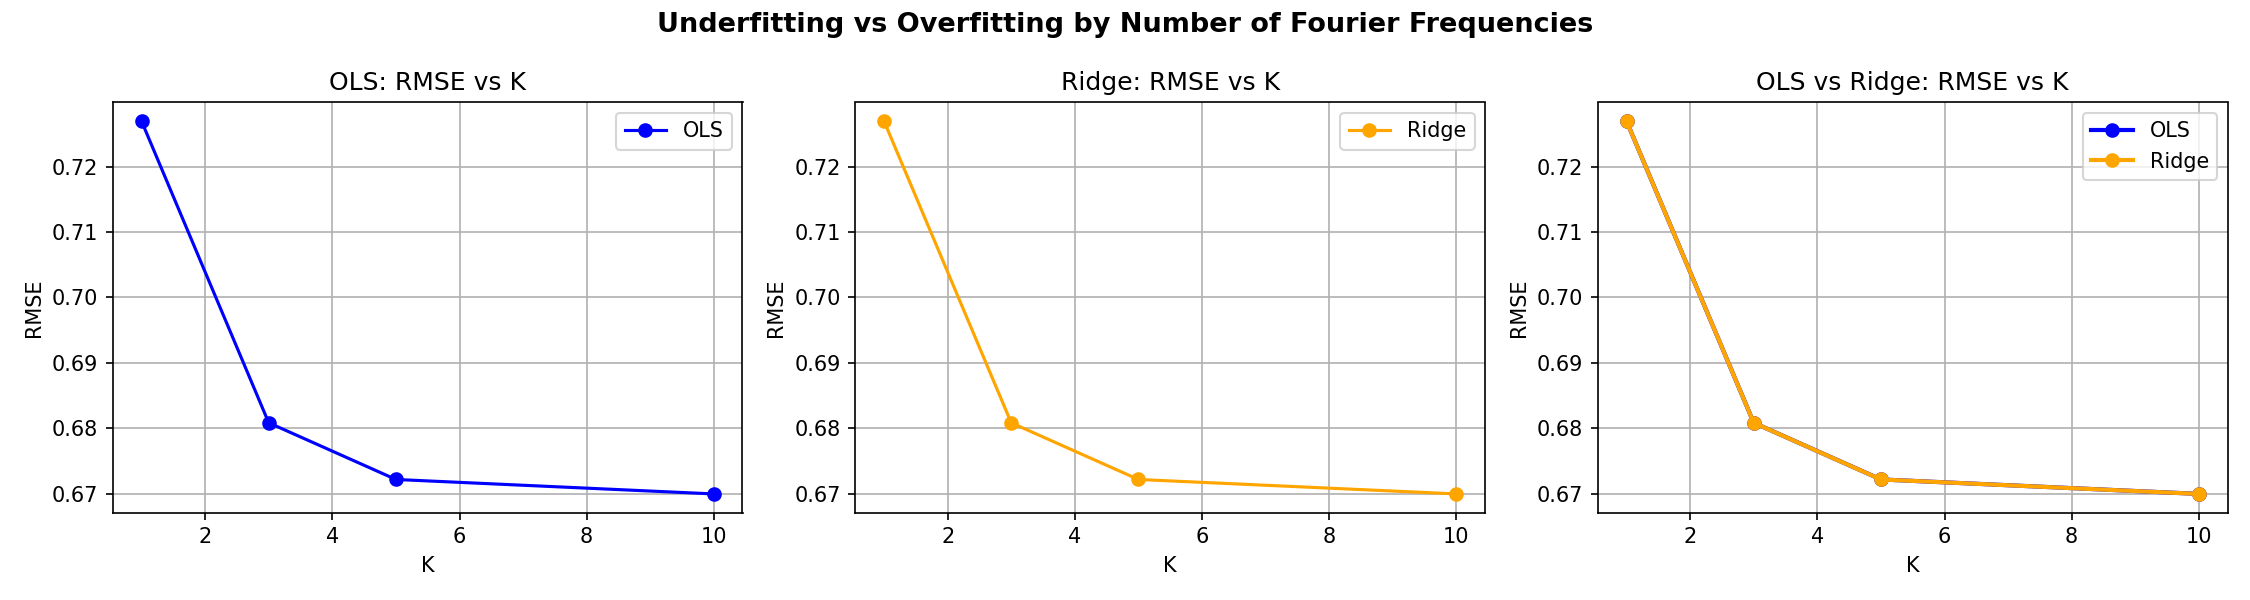
\includegraphics[width=0.98\textwidth]{figures/rmse_vs_K.png}
    \caption{RMSE vs.\ $K$ for OLS and Ridge (hour-only features).}
    \label{fig:rmse_k}
\end{figure}

As shown in Figure~\ref{fig:rmse_k}, RMSE drops significantly from $K=1$ to $K=5$, then plateaus. OLS and Ridge perform identically, indicating no overfitting with hour-only features.

\subsection{Model Comparison}

\begin{table}[H]
\centering
\footnotesize
\setlength{\tabcolsep}{6pt}
\caption{Test set performance for the main Fourier-feature setup.}
\begin{tabular}{lcc}
\toprule
\textbf{Model} & \textbf{RMSE} & \textbf{MAE} \\
\midrule
OLS         & 0.6396 & 0.4902 \\
Ridge       & 0.6396 & 0.4902 \\
Shallow MLP & 0.9056 & 0.7059 \\
\bottomrule
\end{tabular}
\label{tab:results}
\end{table}

\subsection{Predictions vs.\ Actual Values}

\begin{figure}[H]
    \centering
    \begin{subfigure}[b]{0.47\textwidth}
        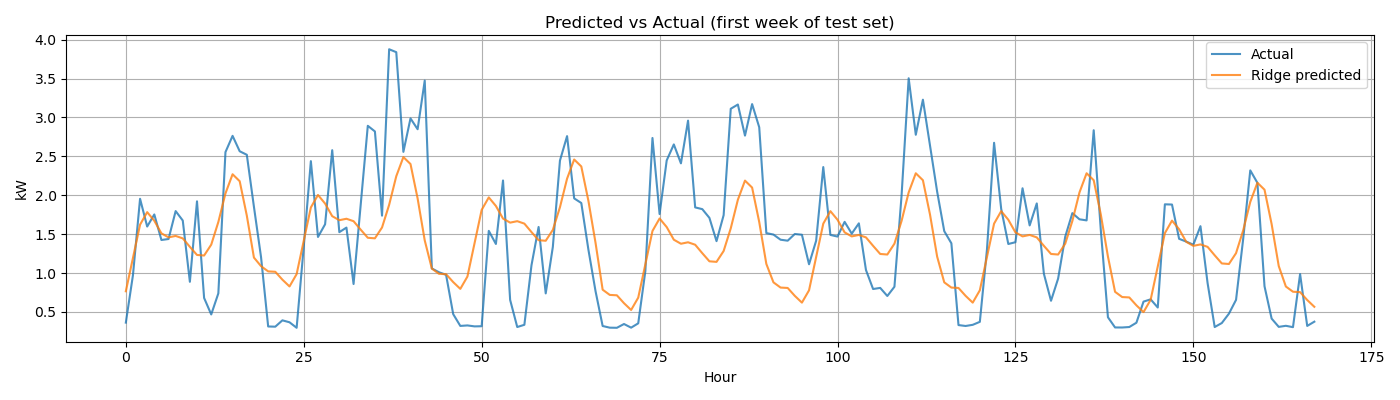
\includegraphics[width=\textwidth]{figures/predictions_vs_actual.png}
        \caption{Ridge regression}
    \end{subfigure}
    \hfill
    \begin{subfigure}[b]{0.47\textwidth}
        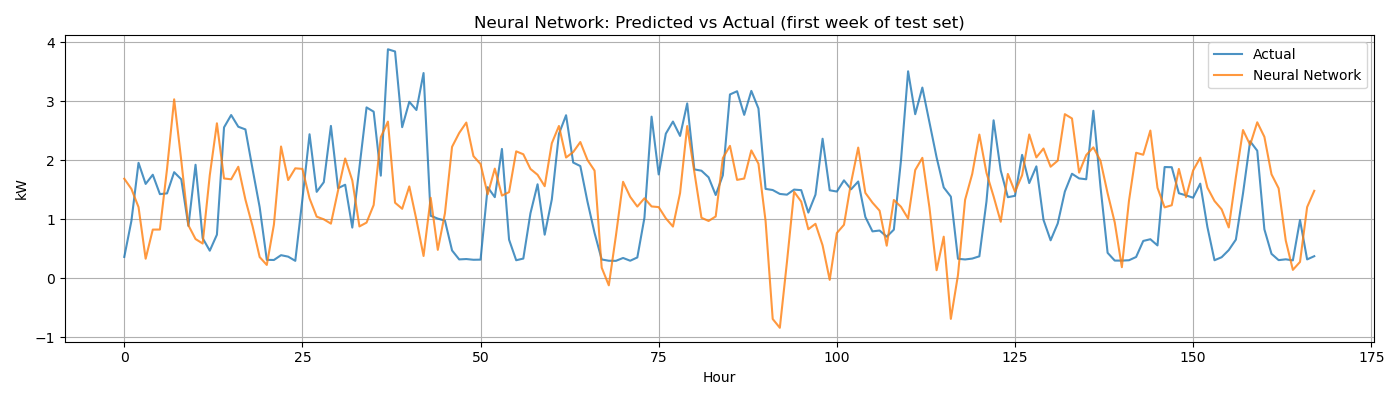
\includegraphics[width=\textwidth]{figures/nn_predictions_vs_actual.png}
        \caption{Shallow MLP}
    \end{subfigure}
    \caption{Predicted vs.\ actual consumption, first week of test set.}
    \label{fig:predictions}
\end{figure}

\subsection{Residual Analysis}

\begin{figure}[H]
    \centering
    \begin{subfigure}[b]{0.47\textwidth}
        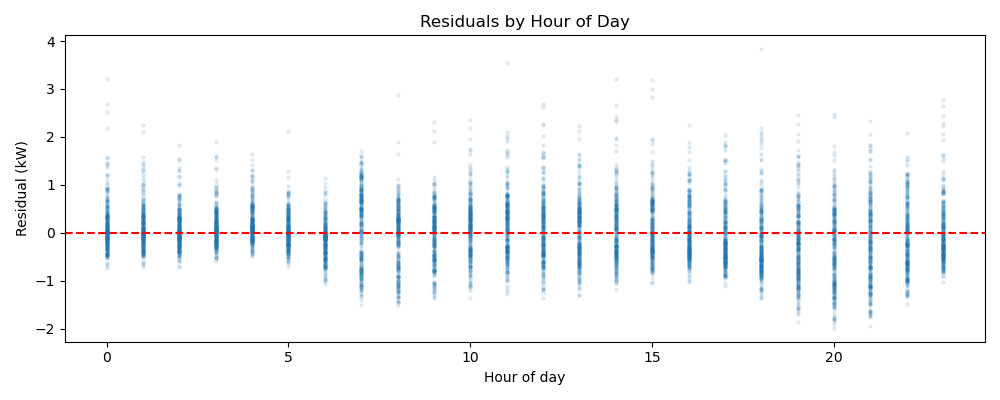
\includegraphics[width=\textwidth]{figures/residuals_by_hour.png}
        \caption{Ridge regression}
    \end{subfigure}
    \hfill
    \begin{subfigure}[b]{0.47\textwidth}
        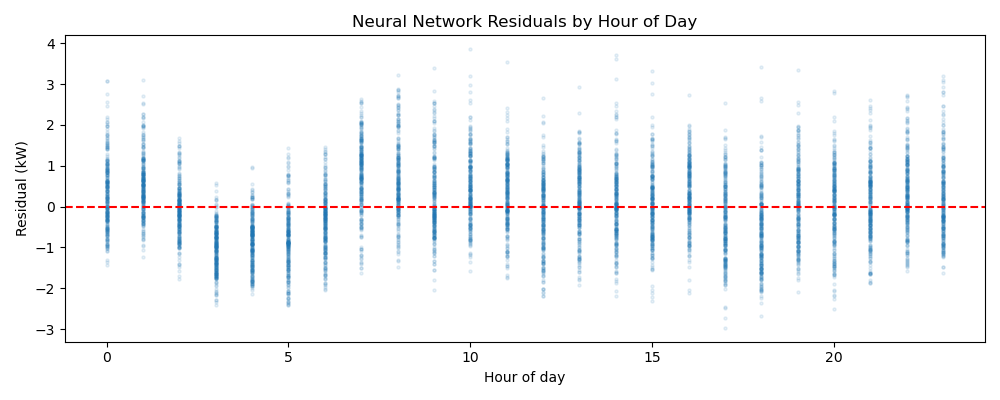
\includegraphics[width=\textwidth]{figures/nn_residuals_by_hour.png}
        \caption{Shallow MLP}
    \end{subfigure}
    \caption{Residuals by hour of day. Errors are centered around zero with no systematic hourly bias.}
    \label{fig:residuals}
\end{figure}

\FloatBarrier



\section{Autoregressive Features}

We investigated whether the inclusion of autoregressive (AR) data improves forecasting accuracy: three time-lagged features (1 hour, 24 hours, 168 hours) and two moving averages (24 hours, 168 hours) were calculated solely based on past values to avoid data leakage. The results showed that this approach improves forecasting accuracy compared to using only Fourier features that reflect calendar time. A ridge regression model was trained using three feature sets: Fourier features only, AR features only, and a combination of both.

\begin{figure}[H]
\centering
\begin{minipage}[c]{0.48\textwidth}
    \centering
    \footnotesize
    \setlength{\tabcolsep}{5pt}
    \begin{tabular}{lcc}
    \toprule
    \textbf{Feature set} & \textbf{RMSE} & \textbf{MAE} \\
    \midrule
    Fourier only & 0.6396 & 0.4898 \\
    AR only      & 0.5235 & 0.3727 \\
    Fourier + AR & 0.5049 & 0.3635 \\
    \bottomrule
    \end{tabular}
    \captionof{table}{Test-set performance by feature set (Ridge, RMSE/MAE in kW).}
    \label{tab:autoregressive}
\end{minipage}%
\hfill
\begin{minipage}[c]{0.48\textwidth}
    \centering
    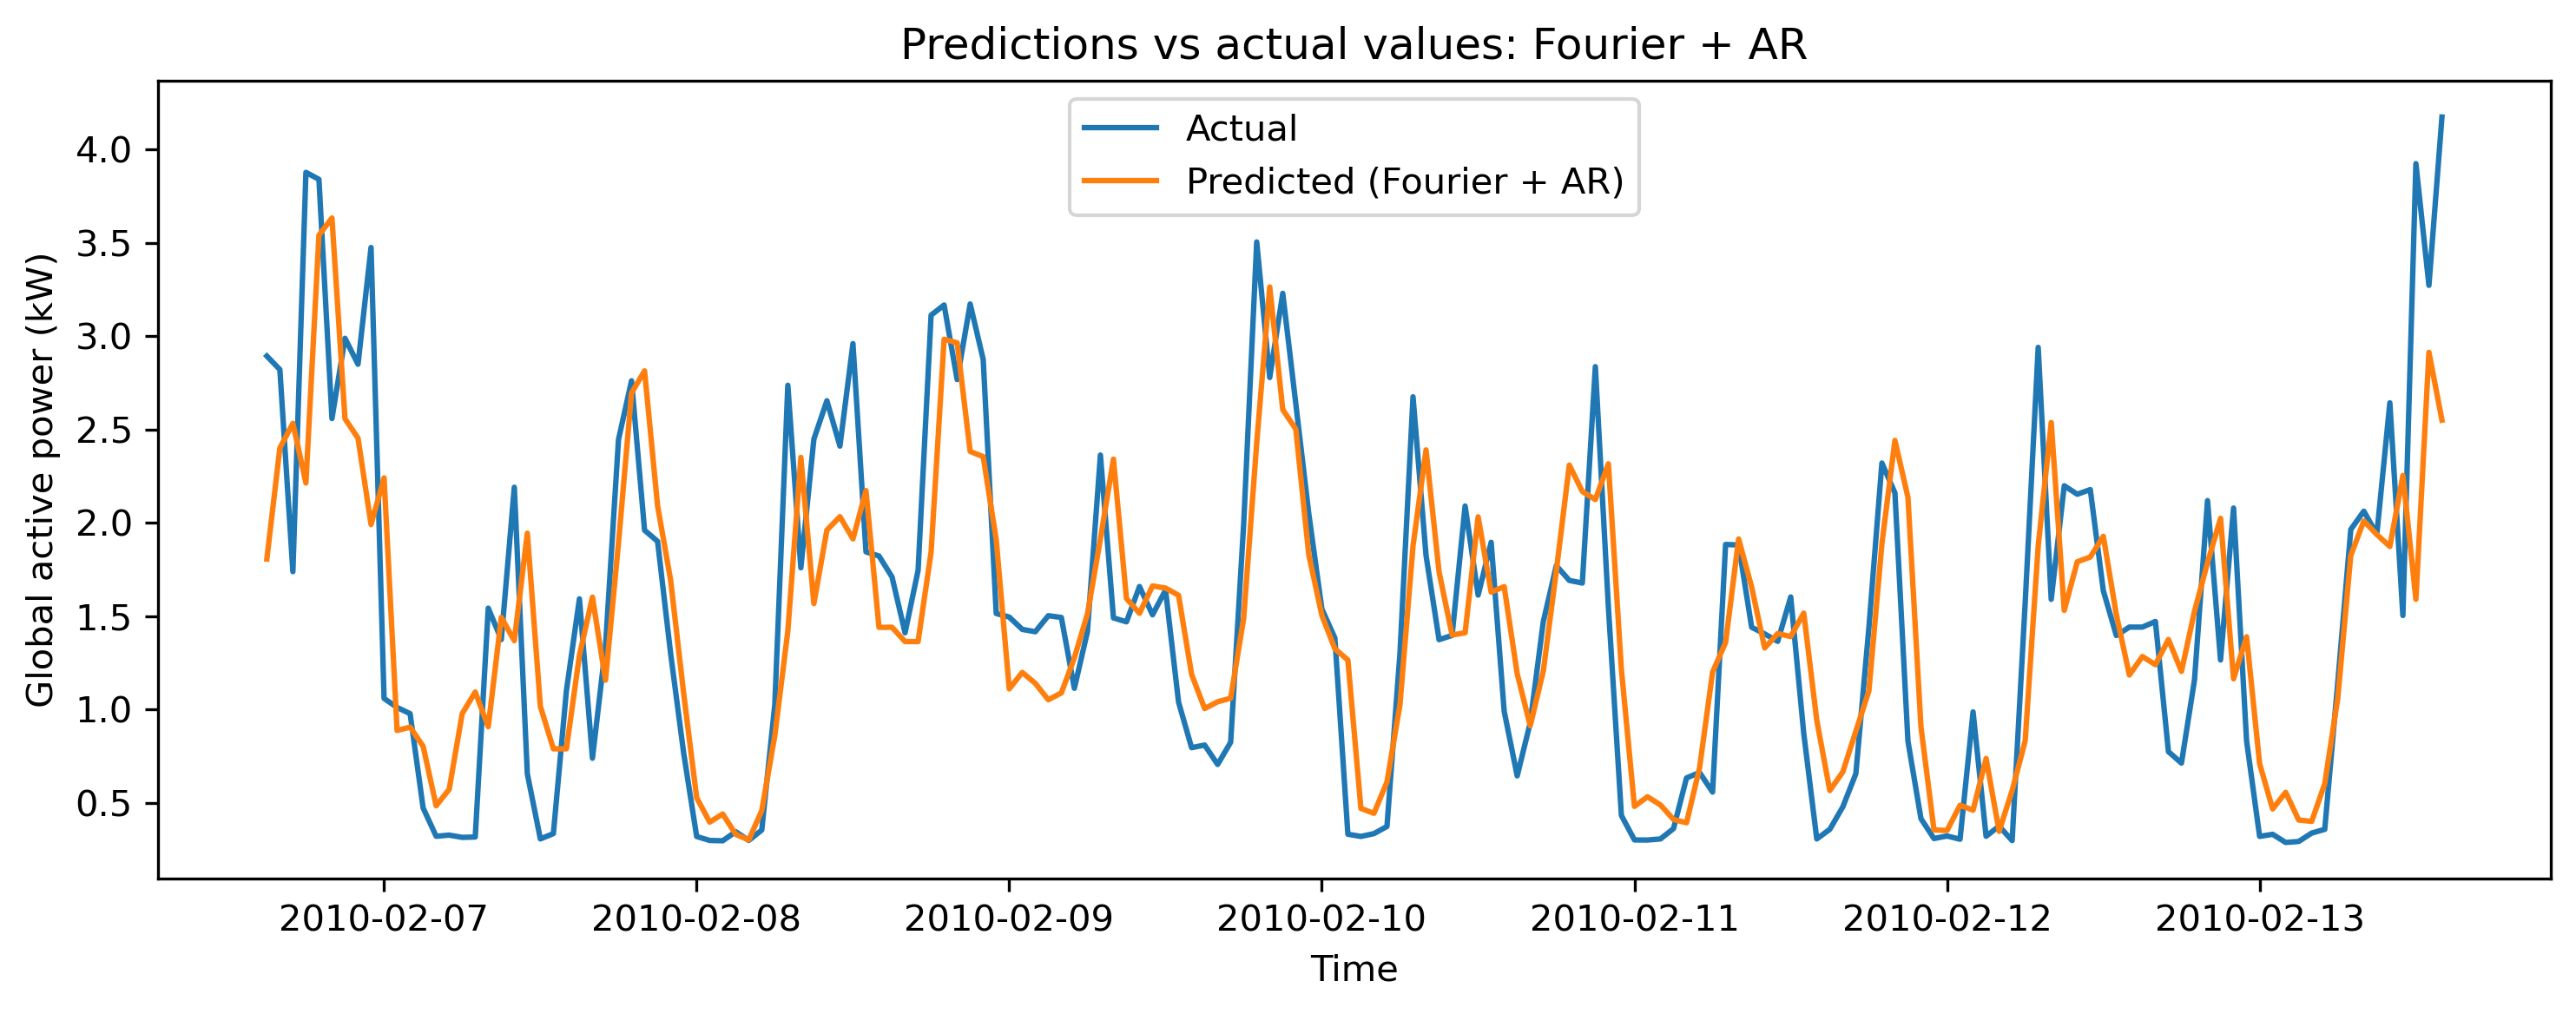
\includegraphics[width=\textwidth]{figures/ar_predictions_vs_actual.png}
    \captionof{figure}{Predicted vs.\ actual consumption, Fourier + AR, first week of test set.}
    \label{fig:ar_predictions}
\end{minipage}
\end{figure}

Including AR features reduced the RMSE by approximately 18\% compared to using Fourier features alone. The combined approach yielded the best results, suggesting that past consumption data contain information that cannot be captured by calendar time alone.

\subsection{Further Analysis}


We additionally tested whether the same Fourier features can predict the three sub-metering signals, using Ridge regression as the best-performing model.



\begin{figure}[H]
\centering
\begin{minipage}[c]{0.55\textwidth}
    \centering
    \footnotesize
    \setlength{\tabcolsep}{4pt}
    \begin{tabular}{lcccc}
    \toprule
    \textbf{Target} & \textbf{Model} & \textbf{K} & \textbf{RMSE} & \textbf{MAE} \\
    \midrule
    Sub-metering 1 & Ridge & 5  & 184.68 & 102.71 \\
    Sub-metering 2 & Ridge & 1  & 204.43 & 91.22  \\
    Sub-metering 3 & Ridge & 10 & 379.65 & 303.76 \\
    \bottomrule
    \end{tabular}
    \captionof{table}{Best test-set performance for sub-metering prediction. RMSE and MAE are measured in Wh.}
    \label{tab:submetering}
\end{minipage}%
\hfill
\begin{minipage}[c]{0.4\textwidth}
    \centering
    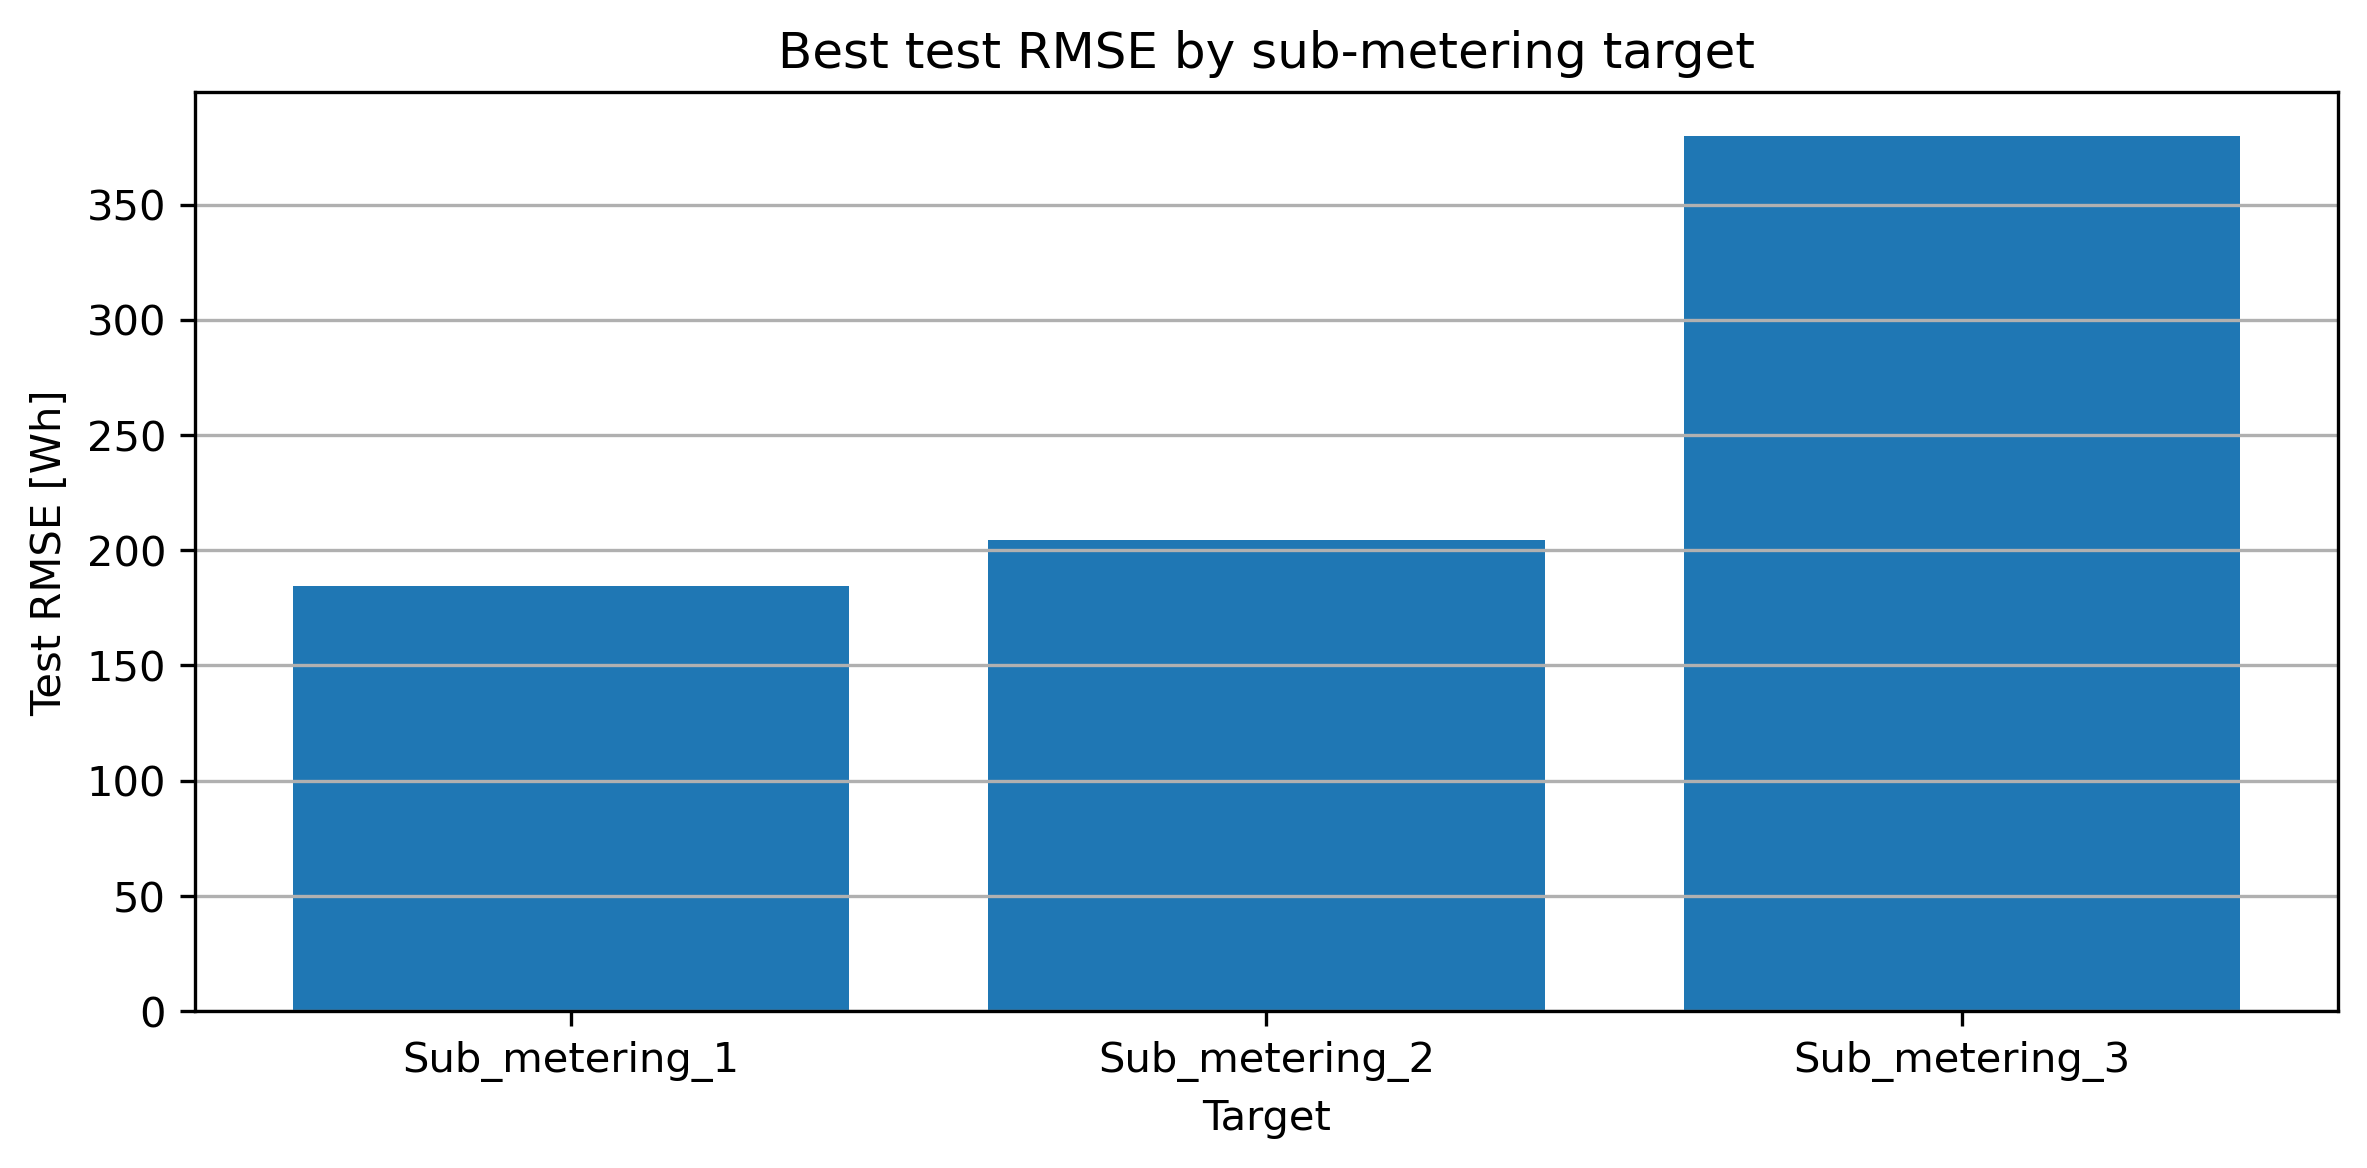
\includegraphics[width=\textwidth]{figures/further_best_test_rmse_by_target.png}
    \captionof{figure}{Best test RMSE for the three sub-metering targets.}
    \label{fig:submetering_rmse}
\end{minipage}
\end{figure}

Sub-metering 1 and 2 are easier to predict from calendar time than Sub-metering 3, suggesting stronger irregular appliance-specific behavior in the third target.



\section{Discussion and Conclusion}

Fourier features based on calendar time capture the key daily, weekly, and seasonal patterns of electricity consumption. OLS and Ridge methods yield nearly identical results (RMSE $=0.64$~kW), outperforming the shallow multilayer perceptron (RMSE $=0.91$~kW). This suggests that Fourier encoding sufficiently linearizes the periodic structure, rendering nonlinear modeling ineffective. Sub-metering analysis confirms that calendar-time features explain the structure even at the individual appliance level, although prediction accuracy varies significantly depending on the target variable.

Incorporating autoregressive terms significantly improves the results obtained using calendar-time features alone: combining lagged and moving-average features with a Fourier basis reduces the Ridge method's root mean square error from $0.64$~kW to $0.50$~kW. This confirms that recent consumption history contains information beyond what is captured by timestamp-encoded data. It also highlights the primary limitation of the purely calendar-time-based approach: it cannot anticipate sudden load spikes caused by household appliances, meaning residual errors remain inevitable, even if the residuals do not exhibit hourly bias. Promising extensions include the use of weather data, extended MLP training with learning rate scheduling, and the application of gradient boosting or RNN models.

\end{document}